\documentclass{article}
\usepackage{amsthm}
\usepackage{graphicx}
\usepackage{rotating}
\usepackage{gensymb}
%\makeatletter
%\def\note{\@ifnextchar[{\@noteWith}{\@noteWithout}}
%\def\@noteWith[#1]{\medbreak\refstepcounter{section}%
%  \renewcommand{\leftmark}{Lecture \thesection}
%  \noindent{\addcontentsline{toc}{section}{Note \thesection: #1\@addpunct{.}}%
%  \sectionfont Note \thesection. #1\@addpunct{.}}\medbreak}
%\def\@noteWithout{\medbreak\refstepcounter{section}%
%  \renewcommand{\leftmark}{Note \thesection}
%  \noindent{\addcontentsline{toc}{section}{Note \thesection.}%
%  \sectionfont Note \thesection.}\medbreak}
%\makeatother

\title{Bellarmine 2017 Eclipse Plans and Notes}

\author{Stephen Brown and Ahktar Mahmood}
\begin{document}

\maketitle


\section{Notes given to us}

\begin{itemize}
\item Provide expert perspective about the upcoming solar eclipse
\item ``How to watch the eclipse"
\item A description of what's happening in the sky
\item What has everyone so excited about this particular opportunity,etc.
\end{itemize}

\section{Additional questions given us}
\begin{enumerate}
\item When the moon blocks direct sunlight, how is that dangerous to the naked eye? What potential dangers should people be aware of when the event occurs?
	\begin{itemize}
	\item Short naked eye viewing (contrary to everything you will hear leading up to the eclipse) is ``mostly" safe. It is highly unlikely that a creature would evolve on a surface of a planet that could be so easily blinded by an item in its normal environment.  In our age of litigious safety concerns, since a lot can harm we are told to never look for any short period. That being sad, ``Don't stare at the Sun."
	\end{itemize}

\item What is the best (or safest) method for viewing a total solar eclipse? Can you offer some general safety tips children and adults can follow?
	\begin{itemize}
	\item	You can look directly at the Sun for brief moments of time.  It is very rare for naked eye viewers to permanently damage their eye-sight in this manner.  The real danger is when using additional larger than our eye optics like binoculars and telescopes.  These gather more light and are correspondingly brighter and are dangerous to look through at the Sun, eclipse or not for any period of time.  Some telescopes have optics that can even be damaged by direct sunlight, and many modern telescopes that are computer controlled have software that doesn't allow the user to even point at the Sun.
	\end{itemize}
\item Are there any dangers in taking photographs or videos? With so many of us carrying smart phones, it will be tempting to video or photograph the occurrence.
	\begin{itemize}
	\item I would feel safe with a smart phone, but with an unfiltered SLR no.  I personally will be taking filtered eclipse pictures with a DSLR camera attached to a computer so I can see the images without having to look through the finder.  I plan to help the other physics faculty to set up something like this at Bellarmine. But mistakes can and will happen (and I have destroyed optics this way) and if you are not comfortable with your equipment, don't do it.  Unless you start to travel to view eclipses, this is most likely a once or twice in a lifetime event, I have never taken or seen a photograph that can transmit the experience, so relish the experience technology free.  I will abandon my attempts at photography if there is any chance it will interfere with the experience.
	\end{itemize}

\item Can Louisville expect total or near-total darkness?
	\begin{itemize}
	\item Surprisingly, there isn't a clear consensus that I could find on this issue.  At Bellarmine, there will be a maximum eclipse of about 95\%, so at maximum you will be able to tell there is definitely something going on, but I have heard stories that people were oblivious during higher eclipses.  But along the center line of the totality, it can be like mid-night and near impossible to ignore.
	\end{itemize}

\item Do you know when the next total solar eclipse will occur?
	\begin{itemize}
	\item Eclipses are visible on a single point of the earth  approximately once every 350 years.  For Louisville, the next one in April of 2024 path will be even closer than this one, but I couldn't find another close one (or even totatlity) for another hundred plus years.
	\end{itemize}

\end{enumerate}

\section{Stephen's notes}

\subsection{Understand!}
MUST BE IN SHADED REGION TO SEE TOTALITY!
\begin{figure}[h]
\centering
\includegraphics[width=85mm]{Pictures/usa_eclipse_map_v2.jpg}
\caption{Total Eclipse Map of United States}
\end{figure}

\begin{sidewaysfigure}
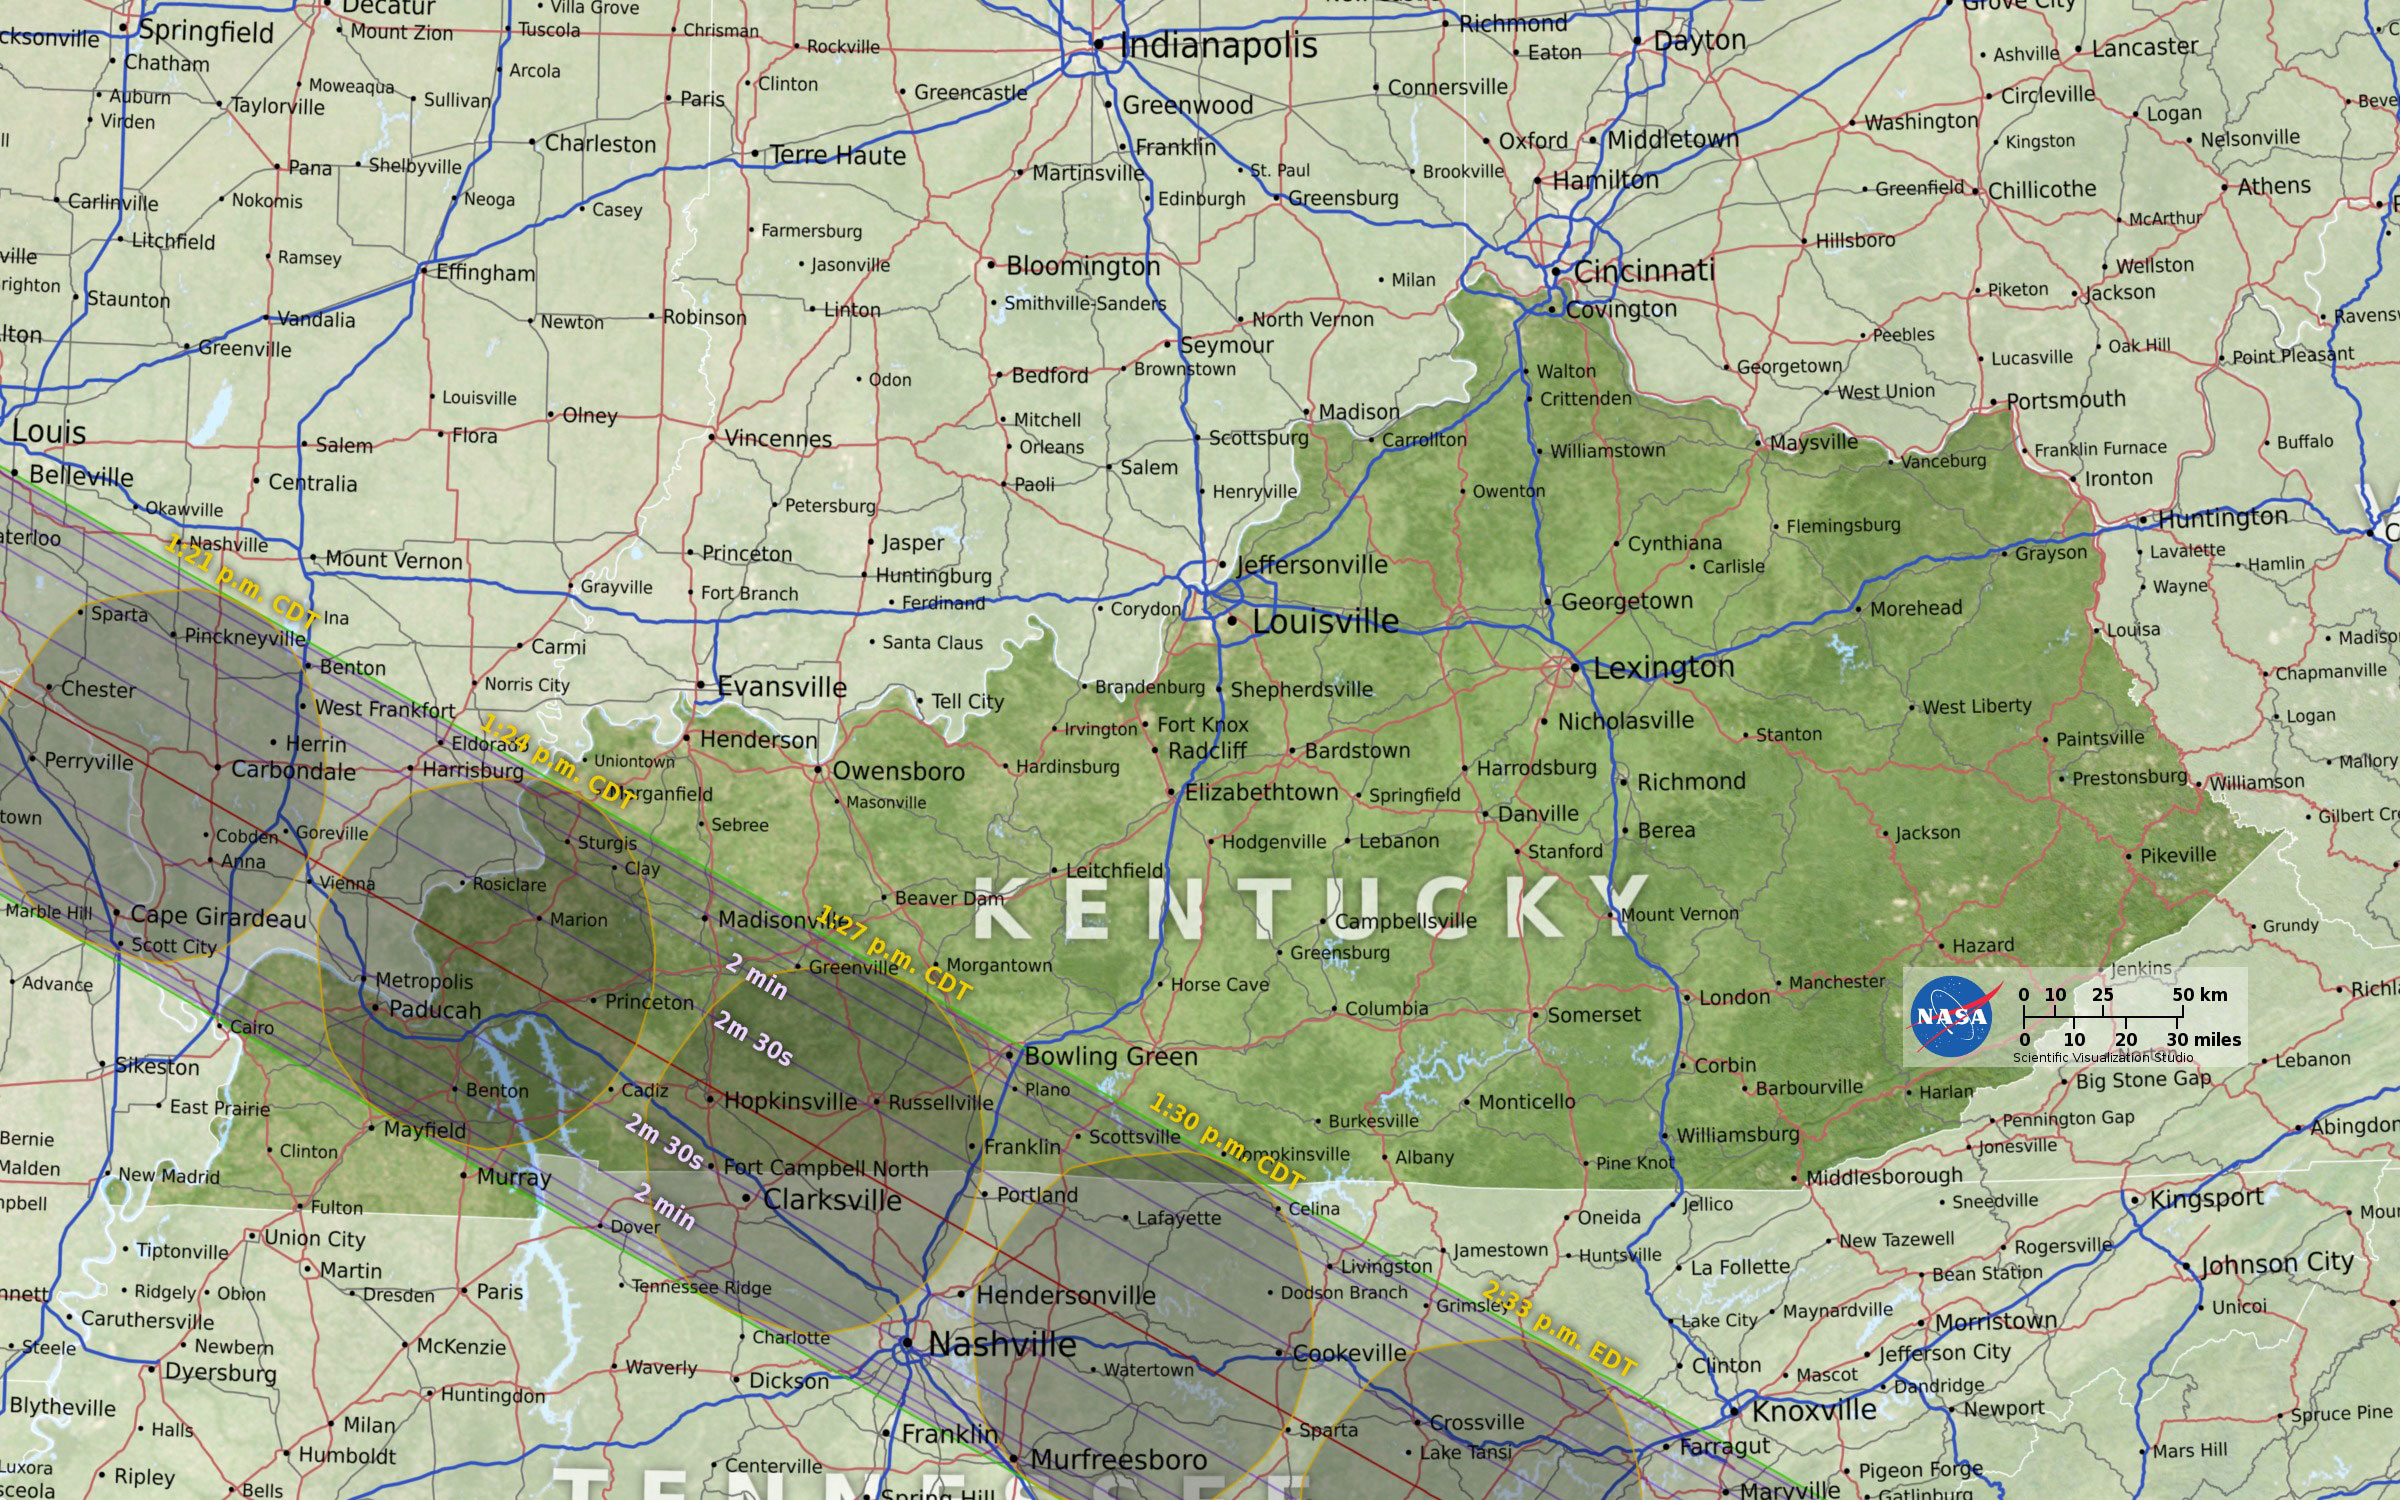
\includegraphics[scale=.3]{Pictures/Ky_eclipse_path.jpg}
\caption{Kentucky's Path of Totality}
\end{sidewaysfigure}

\begin{sidewaysfigure}
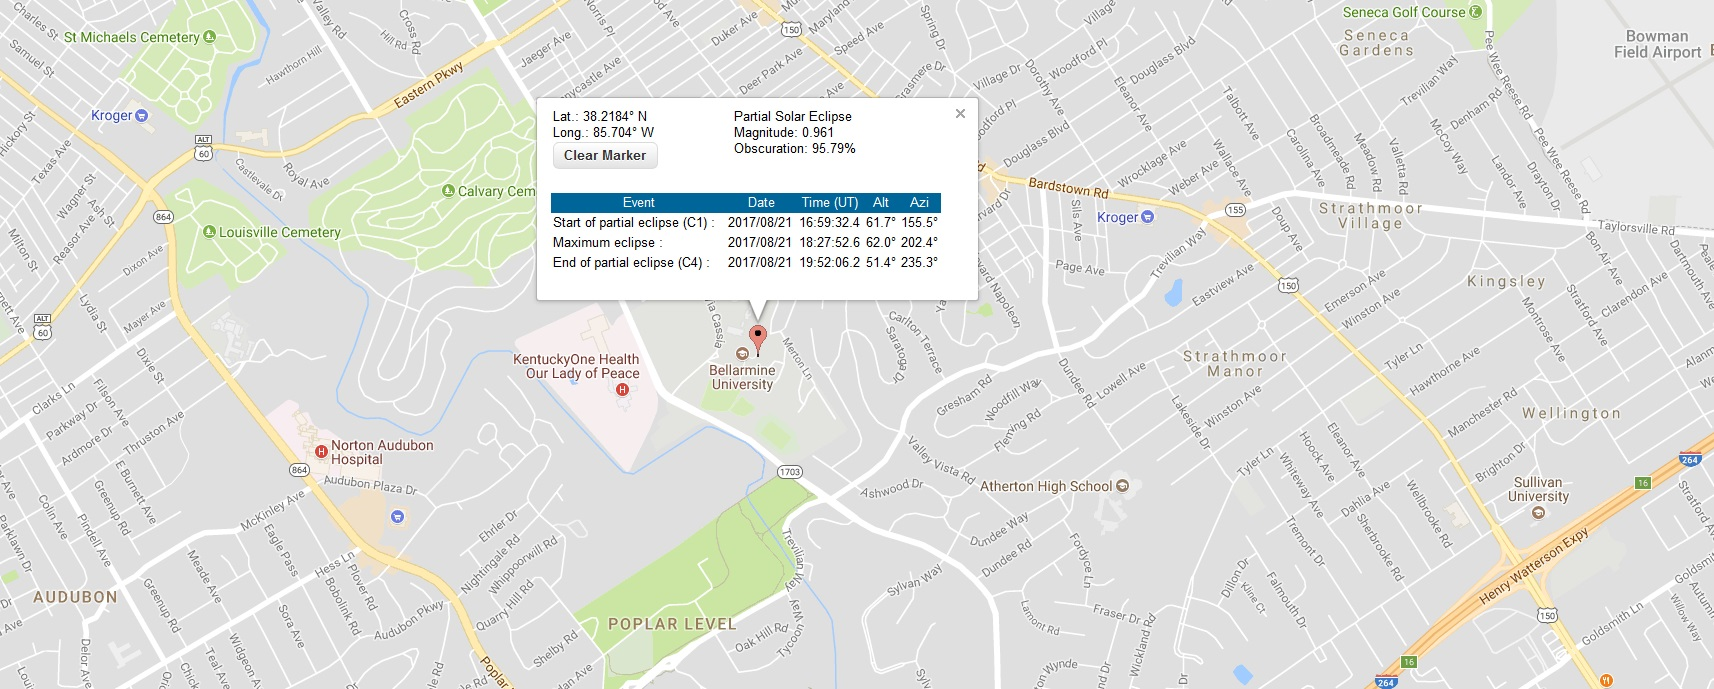
\includegraphics[scale=.9]{Pictures/Local_Bellarmine_Data.jpg}
\caption{Bellarmine's Eclipse Experience Information}
\end{sidewaysfigure}

\begin{sidewaysfigure}
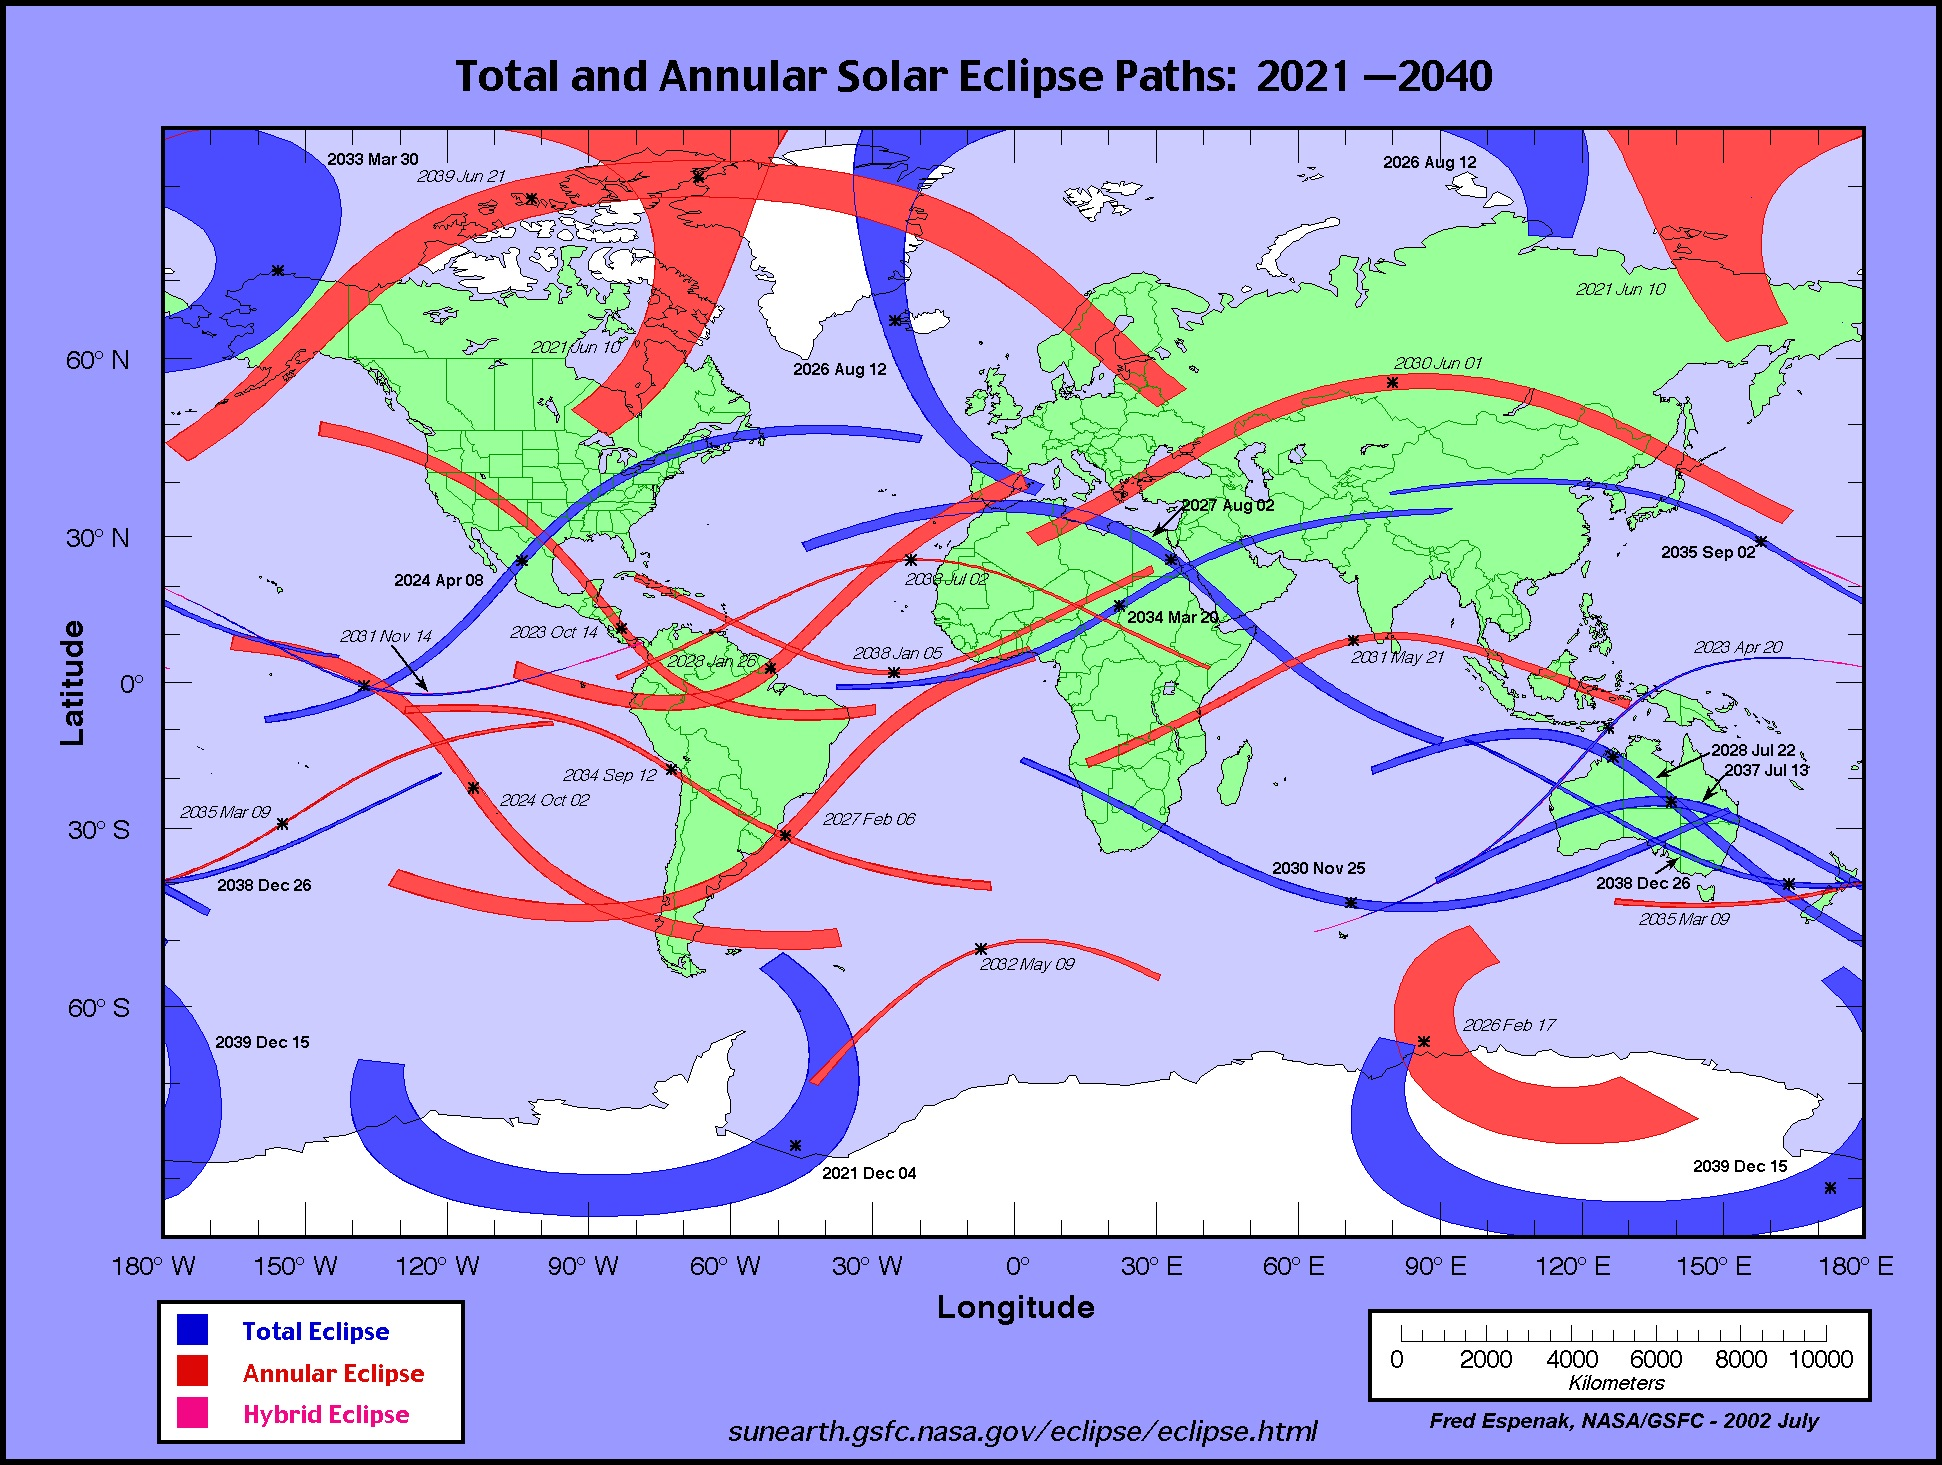
\includegraphics[scale=.75]{Pictures/SEatlas2021.jpg}
\caption{Future eclipse paths}
\end{sidewaysfigure}

\subsection{Next Eclipse}
Next one in the area will be April 2024, but there will not be another total near by till after 2100....so do what you can to see this one.

\subsection{Safety}
\begin{itemize}
\item welding glasses...
\item Don't Look at Sun
\item etc
\end{itemize}

\subsection{What's going on in the Sky?}
\begin{itemize}
\item Saros cylce = 18 yrs, 11 days, 8 hrs.  (120 \degree (...in which directioin I don't know...)  The type of alignment follows the Saros Cycle--although this has no bearing on a local observer.  The spot at which he/she views an eclipse will not have another one in about 350 years.
\item syzygy  "astronomical alignment"
	\begin{itemize}
\item 'all eclipses are syzygy events, but not all syzygy events are eclipses.'
\item The Sun, Moon, and the Earth can line up to 7 times a year
		\begin{itemize}
		\item lunar eclipses are view-able from half the Earth
		\item solar eclipses the viewer must be in the shadow
			\begin{itemize}
			\item partial solar eclipse = viewer is in umbra
			\item total solar eclipse = viewer is in penumbra
			(annular eclipse is a total eclipse and the Moon is farther away than a normal total eclipse so it doesn't cover all the Sun.
			\end{itemize}
		\end{itemize}
	\end{itemize}
\item The Moon is 400 times smaller than the Sun, but is 400 times closer to the Earth. (1/2\degree in angular diameter)
\end{itemize}

\subsection{Things to look for before totality}
\begin{itemize}
\item Shadow Bands.  Bands of shadows that cross the surface.  I've always been in flat locations without height when I've seen eclipses and I never had a chance to see them.  Hopefully, this time I plan to be higher than the local terrain...
\item Baily's Beads.  Sunlight shooting through the valleys and canyons of the Moon right before totality as the higher terrain blocks off sunlight first.  The final one can be a spectacular...
\item Diamond Ring!  The last Baily's Beads can be very brilliant looking like a large diamond shining next to the Sun. 
\end{itemize}

%\begin{figure} [!ht]
%\centering
%\includegraphics[width=85mm]{Figures/Hiperwall_overview.jpg}
%\caption{Hiperwall terminology/topology overview\citep{hiperwallmanual}}
%\label{fig:hp1}
%\end{figure}

\subsection{Bellarmine's Actual Plan for Eclipse}
\begin{itemize}
\item Stephen Brown is NOT going to be doing any outreach!  He will be hopefully encamped in a desolate local free of clouds and with a good view of the surrounding horizon.
\item The solar telescope will be set up in the quad if it is clear.  If the Bellarmine Eclipse Team can get it working, we will have a live camera of the event broadcasting either to the Hiperwall or to a nearby television.
\item The camera will have a solar lens on it and possibly be piggy backed to another telescope with the objective completely blocked off for safety reasons.  This then will be connected to a wifi connected laptop from which it can go to the hiperwall or a hdmi-connected TV. 
\end{itemize}





\end{document}